% Template:     Informe LaTeX
% Documento:    Archivo principal
% Versión:      8.4.4 (02/12/2025)
% Codificación: UTF-8
%
% Autor: Pablo Pizarro R.
%        pablo@ppizarror.com
%
% Manual template: [https://latex.ppizarror.com/informe]
% Licencia MIT:    [https://opensource.org/licenses/MIT]

% CREACIÓN DEL DOCUMENTO
\documentclass[
	spanish, % Idioma: spanish, english, etc.
	letterpaper, oneside
]{article}

% INFORMACIÓN DEL DOCUMENTO
\def\documenttitle {Actividad 1}
\def\documentsubtitle {Actividad 1}
\def\documentsubject {HTTP}

\def\documentauthor {María Moya G., M. Fernando Saavedra}
\def\coursename {Redes}
\def\coursecode {CC4303}

\def\universityname {Universidad de Chile}
\def\universityfaculty {Facultad de Ciencias Físicas y Matemáticas}
\def\universitydepartment {Departamento de Ciencias de la Computación}
\def\universitydepartmentimage {departamentos/dcc}
\def\universitydepartmentimagecfg {height=1.57cm}
\def\universitylocation {Santiago de Chile}

% INTEGRANTES, PROFESORES Y FECHAS
\def\authortable {
	\begin{tabular}{ll}
		Integrantes:
		& \begin{tabular}[t]{l}
			María Moya G. \\
			M. Fernando Saavedra
		\end{tabular} \\
		Profesor:
		& \begin{tabular}[t]{l}
			Ivana Bachmann
		\end{tabular} \\
		Auxiliar:
		& \begin{tabular}[t]{l}
			Julián Ferreira
		\end{tabular} \\
		Ayudantes:
		& \begin{tabular}[t]{l}
			Diego García G. \\
			Valeria Serrano
		\end{tabular} \\
		& \\
		\multicolumn{2}{l}{Fecha de realización: \today} \\
		\multicolumn{2}{l}{Fecha de entrega: 3 de septiembre de 2026} \\
		\multicolumn{2}{l}{\universitylocation}
	\end{tabular}
}

% IMPORTACIÓN DEL TEMPLATE
\input{template}

% CONVENCIÓN TIPOGRÁFICA
% Monoespaciado SOLO para lo que existe literalmente en el código, en el archivo
% de configuración o en el flujo de bytes. Los nombres de headers y los códigos
% de estado HTTP se escriben en texto normal (su forma Capitalizada-Con-Guion ya
% los distingue). Cambiar una sola definición reetiqueta todo el informe.
\newcommand{\code}[1]{\texttt{#1}}    % identificadores, funciones, archivos, comandos
\newcommand{\cfgkey}[1]{\texttt{#1}}  % claves del archivo de configuración JSON
\newcommand{\hdr}[1]{#1}              % nombres de headers HTTP
\newcommand{\status}[1]{#1}           % códigos de estado HTTP

% INICIO DE PÁGINAS
\begin{document}

% PORTADA
\templatePortrait

% CONFIGURACIÓN DE PÁGINA Y ENCABEZADOS
\templatePagecfg

% RESUMEN O ABSTRACT
%\begin{abstractd}
%	\lipsum[1] % Párrafo ejemplo, se puede borrar
%\end{abstractd}

% TABLA DE CONTENIDOS - ÍNDICE
\templateIndex

% CONFIGURACIONES FINALES
\templateFinalcfg

% ======================= INICIO DEL DOCUMENTO =======================

\section{HttpMessage.py}
Se diseña la clase HttpMessage con el objetivo de concentrar la lógica en un solo objeto, siguiendo principios de OOP.
Un programa cliente, servidor o proxy puede enviar o recibir mensajes Http con esta misma clase.

Nuestro método \code{HttpMessage.parse} se encarga de extraer el HEAD del mensaje recibido en bytes, decodificarlo y almacenar cada header con su valor en un HttpMessage.
BODY también se guarda, sin decodificar, en la misma clase. \code{HttpMessage.to\_bytes} hace el camino inverso: serializa un HttpMessage a bytes, listo para enviar por un socket.
\subsection{¿Qué debe extraer \code{parse}?}
Un mensaje HTTP se compone de HEAD y BODY separados por \verb|\r\n\r\n|, donde el HEAD es texto y el BODY no necesariamente.
Siguiendo esa estructura, \code{parse} extrae:

\begin{itemize}
	\item \textbf{Start line}: es la única línea cuyo formato depende de la dirección del mensaje. Si parte con \code{HTTP/} es una respuesta y se extraen \code{version}, \code{status\_code} y \code{reason}; en caso contrario es una request y se extraen \code{method}, \code{path} y \code{version}.
	\item \textbf{Headers}: cada línea restante del HEAD tiene el formato \code{Nombre: valor} y se guarda en un diccionario. Se decidió utilizar un diccionario para facilitar el acceso a los headers por nombre. Para esta actividad importan \hdr{Host} (dominio y puerto del servidor destino, 80 por defecto), \hdr{Content-Length} (cuántos bytes de BODY hay que leer), \hdr{Content-Type} (si el BODY es texto reemplazable o binario) y \hdr{Connection}.
	\item \textbf{Body}: todo lo que sigue al \verb|\r\n\r\n|, sin decodificar, porque puede ser binario (por ejemplo, una imagen).
	\item \textbf{Bytes originales} (\code{raw}): permiten reenviar el mensaje tal como llegó y depurar.
\end{itemize}

La estrategia fue extraer lo que el proxy necesita para decidir y para reconstruir el mensaje: \hdr{Host} y \code{path} para saber a qué servidor conectarse y si está bloqueado, \hdr{Content-Length} para saber cuándo terminó el mensaje cuando el buffer es más pequeño que este, y la start line para rearmar el mensaje o reemplazarla por un \status{403}.

No se extrae ni se normaliza el resto: los nombres de headers se guardan tal como llegan, un header repetido sobrescribe al anterior y se asume \hdr{Content-Length} (no se soporta \hdr{Transfer-Encoding: chunked}).

\subsection{Creación de mensajes}
\code{create\_HTTP\_message} (\code{HttpMessage.to\_bytes}) hace el camino inverso: rearma la start line según si el mensaje es request o response, escribe los headers como \code{Nombre: valor} separados por \verb|\r\n|, cierra el HEAD con \verb|\r\n\r\n| y concatena el BODY en bytes.
Si el mensaje declaraba \hdr{Content-Length}, este se recalcula al serializar, de modo que un BODY editado por el proxy (reemplazo de palabras) mantenga un largo consistente.

\section{server.py}
El servidor de la parte 1 recibe la ruta de su archivo de configuración JSON como argumento (\code{sys.argv}) y de ahí obtiene el nombre del usuario.
Escucha en \code{(0.0.0.0, 8000)}, lee la request con \code{HttpMessage.receive} y responde con un \status{200 OK} que lleva un HTML mínimo, agregando el header \hdr{X-ElQuePregunta} con el nombre leído del JSON.
En la parte 2 este mismo archivo se transforma en el proxy.

Las pruebas de esta primera parte se hicieron sobre la misma máquina virtual: se capturó la request enviada por el navegador a \code{(IP\_VM, 8000)} y se verificó que \code{parse\_HTTP\_message} la interpretaba correctamente, y luego \code{curl -i IP\_VM:8000} devolvió un \status{200 OK} con el HTML y el header \hdr{X-ElQuePregunta} tomado del archivo JSON.

\section{Proxy}

\subsection{Diagrama de flujo y sockets}
El proxy se comporta simultáneamente como servidor (frente al cliente) y como cliente (frente al servidor de origen), por lo que debe mantener dos conexiones abiertas al mismo tiempo.
La Figura \ref{img:proxy} muestra el flujo completo de una transacción, incluyendo la rama en que el dominio está bloqueado.

\insertimage[\label{img:proxy}]{diagrama-proxy.pdf}{width=0.95\textwidth}{Flujo de una transacción a través del proxy y sockets involucrados. La rama roja segmentada corresponde al caso en que el dominio pedido está bloqueado.}

En total el proxy necesita \textbf{tres sockets}, de los cuales solo dos transportan datos:

\begin{itemize}
	\item \textbf{S1, socket de escucha}: se crea una sola vez al iniciar el programa, se enlaza a \code{(IP\_VM, 8000)} con \code{bind} y queda en \code{listen}. No transporta datos; su única función es aceptar conexiones entrantes, y queda disponible para el siguiente cliente apenas se acepta el actual.
	\item \textbf{S2, socket con el cliente}: es el que devuelve \code{accept} cuando un cliente se conecta. Por él llega la request y por él se envía la respuesta final. Sobre este socket el proxy actúa como servidor.
	\item \textbf{S3, socket con el servidor de origen}: lo crea el proxy con \code{connect} hacia \code{(host, 80)} una vez que sabe cuál es el destino. Sobre este socket el proxy actúa como cliente.
\end{itemize}

S1 vive durante toda la ejecución, mientras que S2 y S3 se crean y se cierran una vez por transacción.
S3 además es condicional: si el dominio pedido está en la lista \cfgkey{blocked} del archivo de configuración, el proxy responde el \status{403} por S2 con contenido generado localmente y S3 nunca llega a crearse, de modo que el servidor prohibido nunca recibe la petición.

\subsection{Obtención de la dirección del servidor destino}
El proxy no tiene la dirección del servidor configurada de antemano: la deduce del propio mensaje HTTP que recibe.
Cuando un cliente está configurado para usar un proxy, abre la conexión TCP contra el proxy, pero escribe el destino real dentro de la request en forma absoluta: la start line lleva la URL completa del destino en vez de solo el path, y además se incluye el header obligatorio \hdr{Host} (ver el bloque siguiente).
Cualquiera de las dos fuentes sirve; en nuestra implementación usamos el header \hdr{Host}.
De esa autoridad se obtiene el par \code{(host, puerto)}, separando el puerto si viene explícito como \code{host:puerto} y asumiendo el puerto canónico 80 en caso contrario.
Con ese par se hace \code{connect} del socket S3, sin necesidad de resolver el dominio manualmente, ya que \code{socket.connect} acepta el nombre de dominio y realiza la resolución DNS internamente.
Nótese que el cliente sí conoce el destino ---es quien lo eligió---, pero no establece ninguna conexión con él ni resuelve su IP: ambas cosas las hace el proxy en su nombre, y es justamente esto lo que le permite filtrar o bloquear el acceso.

La diferencia entre ambas formas se puede observar capturando con un socket lo que envía \code{curl}:

\begin{verbatim}
% curl example.com -x IP_VM:8000        (forma absoluta, hacia el proxy)
GET http://example.com/ HTTP/1.1
Host: example.com

% curl http://IP_VM:8000/index.html     (forma origen, sin proxy)
GET /index.html HTTP/1.1
Host: IP_VM:8000
\end{verbatim}

\subsection{Bloqueo de dominios prohibidos}
La detección de dominios bloqueados se realiza leyendo desde el archivo JSON la clave \cfgkey{blocked}, que contiene los dominios que no están permitidos. Cuando llega una petición HTTP se obtiene el dominio desde el header \hdr{Host}, de la forma antes descrita, y se construye la URL completa. Luego, el proxy recorre la lista de dominios bloqueados y verifica si alguno está contenido en la URL solicitada: de encontrarse una coincidencia, la petición es bloqueada y el proxy responde directamente al cliente con un \status{403 Forbidden}. La respuesta contiene un HTML que incluye una etiqueta \verb|<img src="/gato.jpg">|, indicando al navegador que debe solicitar la imagen. Esta segunda solicitud, cuyo path es \code{/gato.jpg}, debe ser reconocida por el proxy antes de intentar reenviarla al servidor de destino, ya que la imagen se encuentra almacenada localmente en el proxy y no en el servidor solicitado originalmente. Por lo tanto el proxy detecta esta ruta, busca el archivo \code{gato.jpg} localmente y responde directamente al navegador con la imagen, evitando que la solicitud sea enviada al servidor de destino.

Luego, para poder mostrar la imagen se necesitan 2 ciclos de comunicación HTTP: primero, un ciclo para solicitar y recibir la página HTML bloqueada (con el \status{403}), y luego un segundo ciclo en el que el navegador solicita \code{/gato.jpg} y el proxy le responde con la imagen almacenada localmente.

\subsection{Header X-ElQuePregunta}
Cuando el destino no está bloqueado, el proxy agrega a la petición el header \hdr{X-ElQuePregunta}, cuyo valor corresponde al nombre del usuario obtenido desde el archivo JSON. Esto se realiza antes de reenviar la petición al servidor destino, mediante \code{request\_msg.headers["X-ElQuePregunta"] = user\_name}. Luego el proxy envía la petición modificada al servidor a través del socket correspondiente.

\subsection{Reemplazo de palabras prohibidas}
Una vez recibida la respuesta del servidor destino, el proxy revisa su BODY para reemplazar las palabras indicadas en la clave \cfgkey{forbidden\_words} del archivo JSON. Para esto primero convierte el BODY desde bytes a texto utilizando UTF-8, luego, recorre las palabras prohibidas y reemplaza cada una por el texto correspondiente. Finalmente convierte nuevamente el BODY modificado a bytes antes de enviarlo al cliente.

Es necesario recalcular el \hdr{Content-Length} después del reemplazo, ya que este header indica la cantidad de bytes que contiene el BODY. Como el reemplazo puede cambiar el tamaño del contenido, el valor original de \hdr{Content-Length} podría dejar de coincidir con la cantidad real de bytes del BODY. Por lo tanto se debe actualizar con el nuevo tamaño antes de enviar la respuesta al cliente.

\subsection{Recepción con buffer pequeño}
La función \code{HttpMessage.\_read\_raw} realiza la recepción del mensaje en dos fases: primero se leen los bytes necesarios para obtener los headers, identificando el final de esta sección mediante la secuencia \verb|\r\n\r\n|. Una vez obtenidos los headers, se determina la cantidad de bytes del BODY a partir del header \hdr{Content-Length}, y se continúa leyendo hasta recibir la cantidad indicada.

Para saber si el mensaje completo llegó se debe haber recibido el final de los headers y, si existe un BODY, la cantidad de bytes indicada por \hdr{Content-Length}. Si los headers no caben en un solo buffer se realizan múltiples lecturas y se van acumulando los bytes recibidos hasta encontrar \verb|\r\n\r\n|. De esta forma, el tamaño del buffer no determina el tamaño máximo de los headers.

La sección de headers se considera completa al encontrar \verb|\r\n\r\n|. En cuanto al BODY, se considera completo cuando se han recibido exactamente los bytes indicados por \hdr{Content-Length}. Por lo tanto, tanto los headers como el BODY pueden requerir varias llamadas a \code{recv()} cuando se utiliza un buffer pequeño.

\section{Pruebas}
Todas las pruebas se ejecutaron con el proxy corriendo en la máquina virtual, con su socket de escucha enlazado a \code{(0.0.0.0, 8000)} y accedido desde la máquina anfitriona como \code{IP\_VM:8000}; en las pruebas reportadas \code{IP\_VM} fue \code{192.168.2.5}. Antes de configurar el proxy se verificó que los tres sitios de referencia (\url{http://cc4303.bachmann.cl/}, \url{http://cc4303.bachmann.cl/replace} y \url{http://cc4303.bachmann.cl/secret}) se visualizaban correctamente de forma directa.

\subsection{Pruebas con curl}
\begin{enumerate}
	\item \textbf{Transferencia íntegra:} pedir \url{http://example.com} con y sin proxy entrega
	      exactamente los mismos bytes ---559 en ambos casos, mismo \code{md5sum}---, lo que
	      confirma que el proxy reenvía la request y la response sin alterarlas.

	      \begin{verbatim}
% curl -s example.com | md5sum
c35dafa74975d89a1236a2591acb3616  -
% curl -s example.com -x IP_VM:8000 | md5sum
c35dafa74975d89a1236a2591acb3616  -
	      \end{verbatim}

	      Nótese que \url{http://example.com} responde con \hdr{Transfer-Encoding: chunked} y sin
	      \hdr{Content-Length}; el proxy reenvía el BODY tal como llegó, de modo que el cliente
	      recibe los mismos bytes. La Figura~\ref{fig:curlexample} muestra la comparación completa.

	      \begin{figure}[H]
		      \centering
		      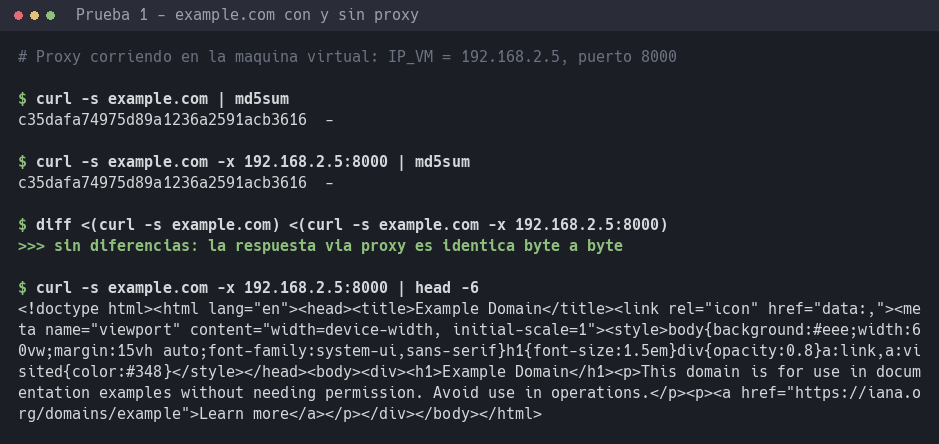
\includegraphics[width=0.8\textwidth]{img/curl-example.png}
		      \caption{Salida de consola: \url{http://example.com} pedido con y sin proxy.}
		      \label{fig:curlexample}
	      \end{figure}

	\item \textbf{Bloqueo de dominios prohibidos:} las dos entradas de \cfgkey{blocked} responden
	      \status{403 Forbidden} sin contactar al servidor de destino, mientras que un sitio no
	      bloqueado sigue respondiendo \status{200 OK}.

	      \begin{verbatim}
% curl -si cc4303.bachmann.cl/secret -x IP_VM:8000
HTTP/1.1 403 Forbidden
Content-Type: text/html; charset=utf-8
Content-Length: 167

<html><body><h1>403 Forbidden - Acceso Prohibido</h1><p>El acceso a esta
ruta esta bloqueado por el proxy.</p><img src='/gato.jpg'></body></html>

% curl -s -o /dev/null -w '%{http_code}' www.dcc.uchile.cl  -x IP_VM:8000
403
% curl -s -o /dev/null -w '%{http_code}' cc4303.bachmann.cl -x IP_VM:8000
200
	      \end{verbatim}

	      El segundo ciclo HTTP se verificó por separado: la petición a \code{/gato.jpg} devuelve
	      \status{200 OK} con \hdr{Content-Type} \code{image/jpeg} y los 89.818 bytes de la imagen
	      local, idénticos al archivo en disco.

	\item \textbf{Header X-ElQuePregunta:} el mensaje de bienvenida cambia al pasar por el proxy,
	      lo que confirma que el header se agrega a la request antes de reenviarla al destino.

	      \begin{verbatim}
% curl -s cc4303.bachmann.cl
    <h1>Bienvenide ... oh? no puedo ver tu nombre :c!</h1>
% curl -s cc4303.bachmann.cl -x IP_VM:8000
    <h1>Bienvenide Maria Elena Moya!</h1>
	      \end{verbatim}

	\item \textbf{Reemplazo de palabras prohibidas:} en \code{/replace} las tres palabras de
	      \cfgkey{forbidden\_words} son reemplazadas y el resto del contenido queda intacto: un
	      \code{diff} contra la misma página pedida sin proxy muestra diferencias únicamente en
	      esas palabras. El BODY original mide 1155 bytes y el reemplazado 1225, y el
	      \hdr{Content-Length} entregado al cliente coincide con este último valor, por lo que el
	      navegador no reporta errores de contenido.

	      \begin{verbatim}
% curl -s cc4303.bachmann.cl/replace -x IP_VM:8000
    <h2>Un [REDACTED] es cualquier dispositivo intermedio entre un cliente
    y servidor ... usando el [REDACTED] del [FORBIDDEN] ... a una [???] a
    la cual la Universidad tiene acceso ...
	      \end{verbatim}

	\item \textbf{Método HEAD (limitación conocida):} \code{curl -I} a través del proxy no llega a
	      completarse. Una respuesta a HEAD no trae BODY, pero sí declara el \hdr{Content-Length}
	      que tendría la respuesta a un GET; como \code{\_read\_raw} solo ve la response y no el
	      método pedido, entra a leer un BODY que nunca llega y queda bloqueado en \code{recv()}
	      hasta que el servidor cierre la conexión. Como el servidor responde
	      \hdr{Connection: keep-alive}, esa espera dura lo que dure su \textit{keep-alive}
	      (cerca de un minuto en nuestras pruebas) y, al ser el proxy de un solo hilo, durante ese
	      lapso no atiende a ningún otro cliente. Se corregiría pasando el método de la request a
	      \code{HttpMessage.receive}, para omitir la lectura del BODY cuando la respuesta
	      corresponde a un HEAD.
\end{enumerate}

\subsection{Pruebas con el navegador}
Las siguientes pruebas se realizaron con el navegador configurado para utilizar el proxy HTTP. Se obtuvieron las siguientes observaciones:

\begin{enumerate}
	\item \textbf{\url{http://cc4303.bachmann.cl/secret}:} la página ya no se muestra,
	      ya que el proxy detecta la ruta bloqueada según la configuración del archivo JSON
	      y responde directamente con un \status{403 Forbidden}, sin contactar al servidor
	      destino. La respuesta contiene un HTML generado por el proxy que incluye una
	      referencia a \code{/gato.jpg}. El navegador realiza una segunda solicitud para
	      obtener dicha imagen, a la cual el proxy responde directamente con la imagen
	      almacenada localmente.

	      En la Figura~\ref{fig:forbidden} se observa la respuesta \status{403 Forbidden}
	      junto con la imagen local.

	      \begin{figure}[H]
		      \centering
		      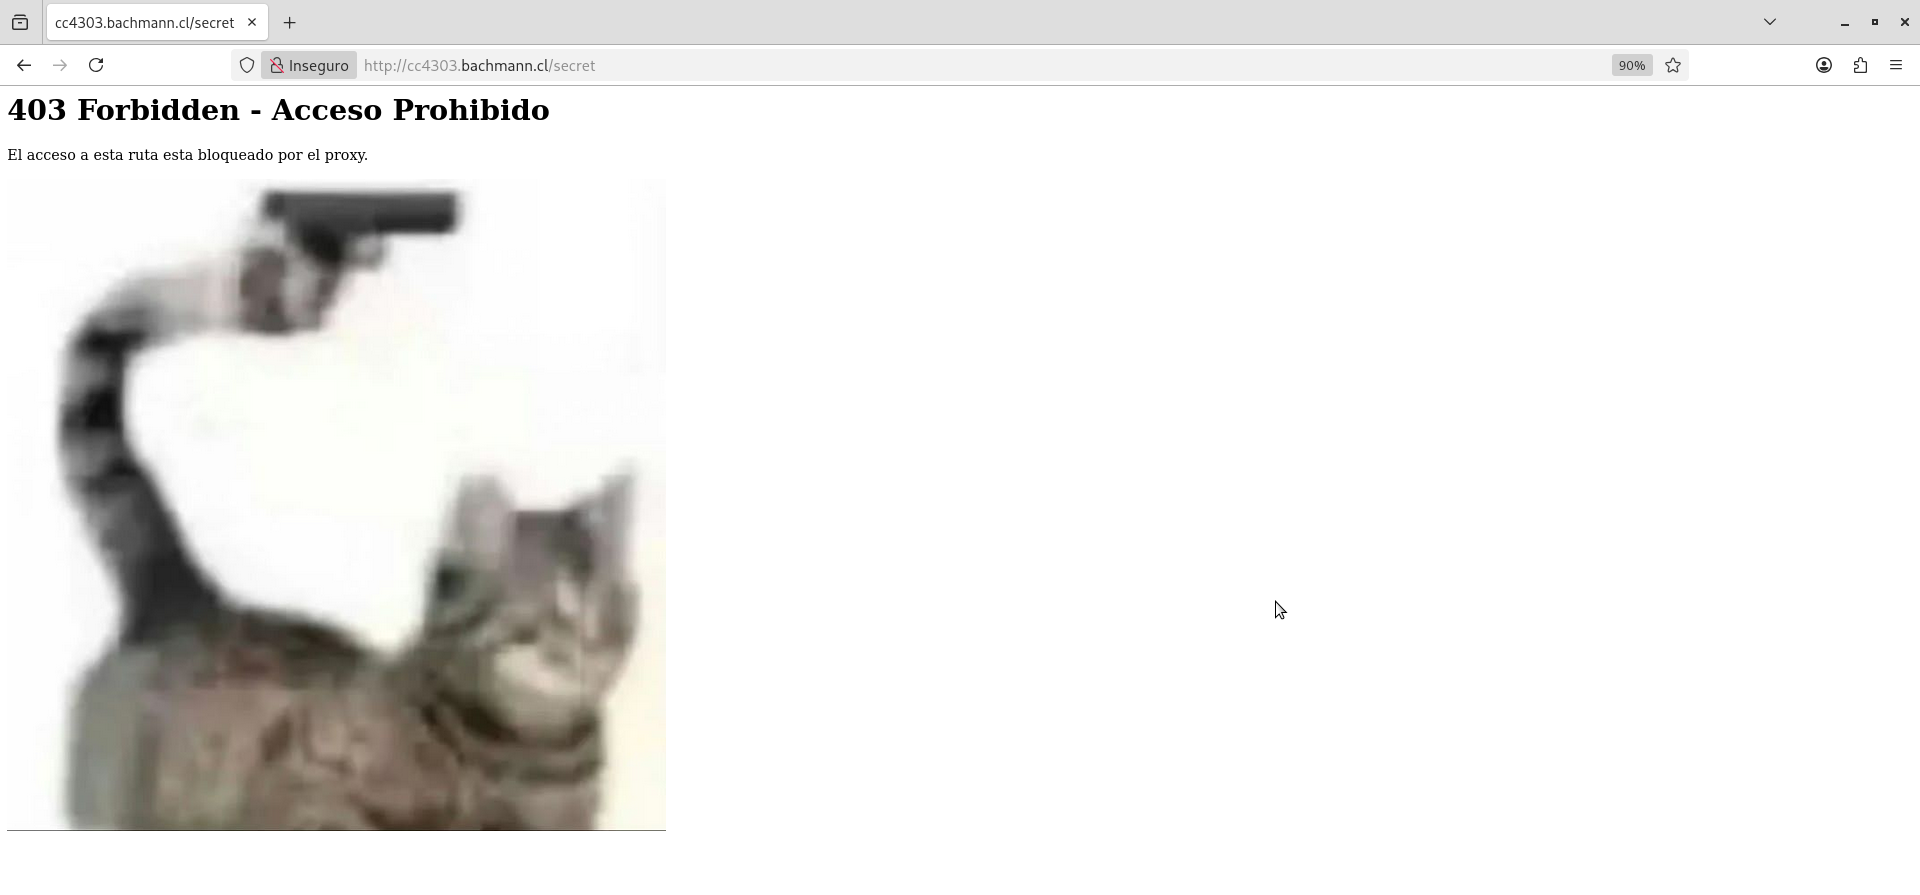
\includegraphics[width=0.8\textwidth]{img/forbidden.png}
		      \caption{Respuesta 403 Forbidden y despliegue de la imagen local.}
		      \label{fig:forbidden}
	      \end{figure}

	\item \textbf{\url{http://cc4303.bachmann.cl/}:} el contenido recibido permite
	      comprobar que el proxy modificó la petición antes de reenviarla al servidor
	      destino. En particular, se agrega el header
	      \hdr{X-ElQuePregunta}, cuyo valor corresponde al nombre obtenido desde el
	      archivo de configuración JSON. El servidor utiliza este header para generar
	      contenido diferente en la respuesta, mostrando el \cfgkey{user\_name} definido en \code{config.json}.

	      La Figura~\ref{fig:header} muestra el resultado obtenido al acceder al sitio,
	      verificando que el header fue agregado correctamente.

	      \begin{figure}[H]
		      \centering
		      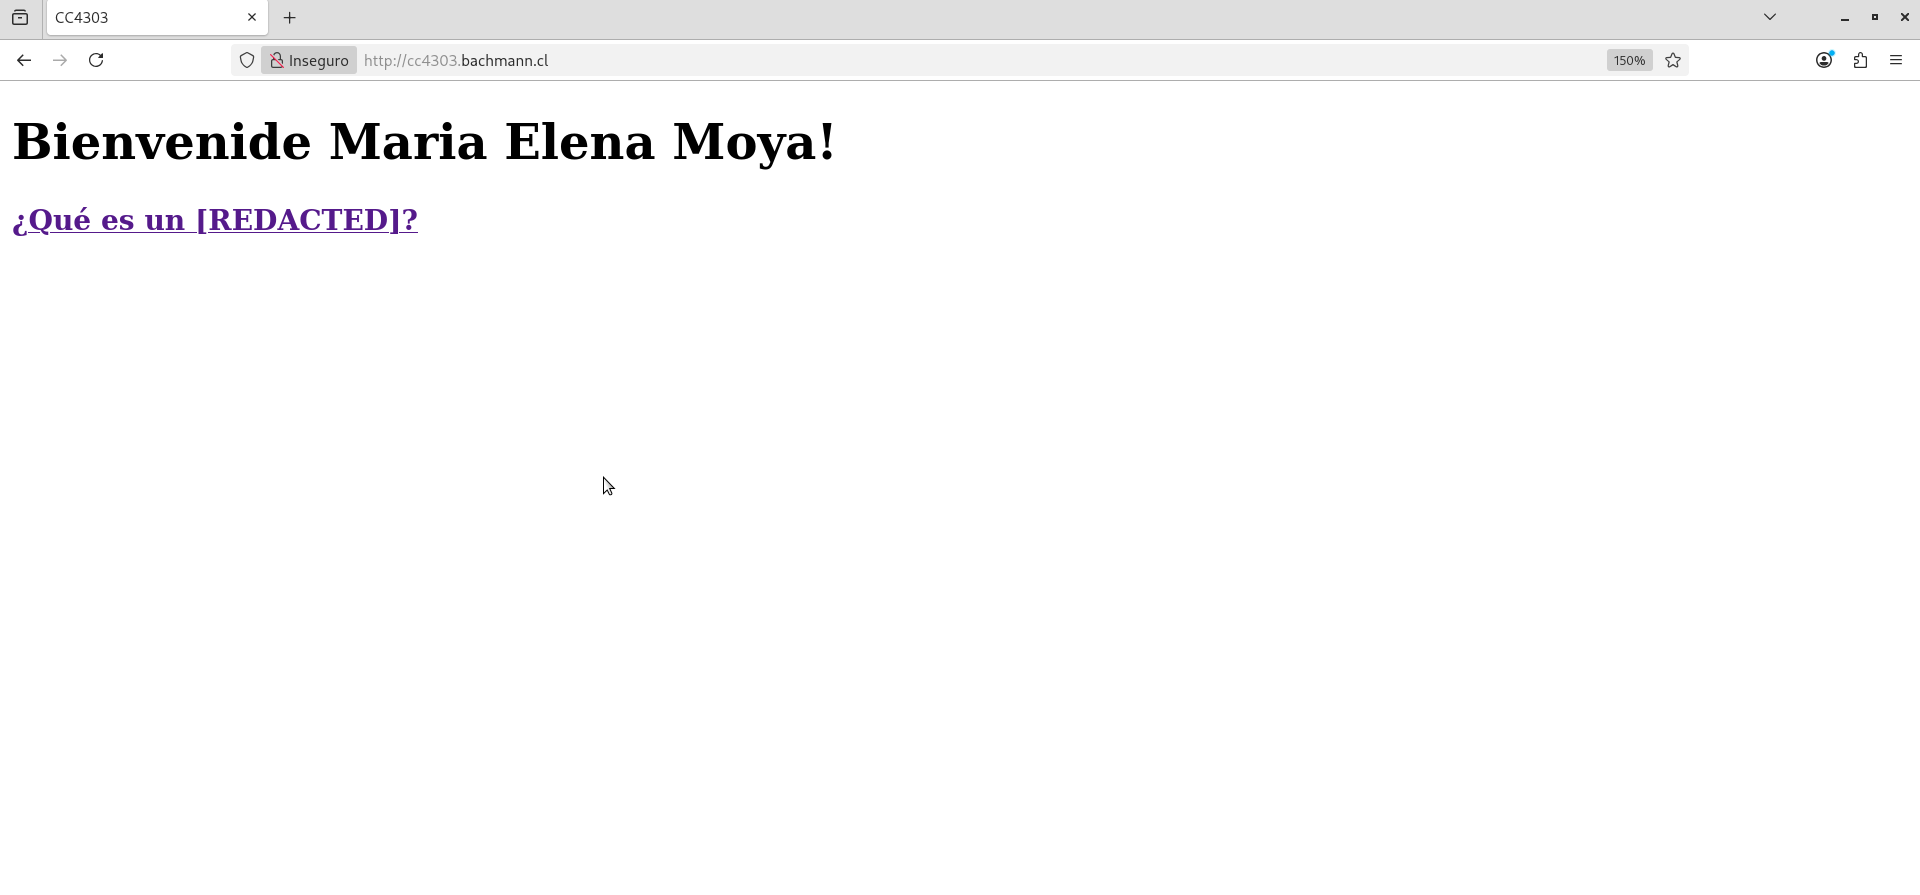
\includegraphics[width=0.8\textwidth]{img/header.png}
		      \caption{Contenido modificado según el header \hdr{X-ElQuePregunta}.}
		      \label{fig:header}
	      \end{figure}

	\item \textbf{Páginas \url{http://cc4303.bachmann.cl/} y \url{http://cc4303.bachmann.cl/replace}:} ambas
	      páginas pueden visualizarse correctamente a través del proxy. Como se observa
	      en la Figura~\ref{fig:header}, la página principal se muestra correctamente, reemplazando la palabra proxy con [REDACTED], mientras que en la Figura~\ref{fig:replace} se observa la versión correspondiente
	      a \code{/replace}. En ambas páginas, el contenido se mantiene salvo por las palabras incluidas en \cfgkey{forbidden\_words}, que
	      son reemplazadas por los valores definidos en el archivo JSON. Esto demuestra
	      que el proxy modifica el BODY de la respuesta antes de enviarlo al navegador.

	      \begin{figure}[H]
		      \centering
		      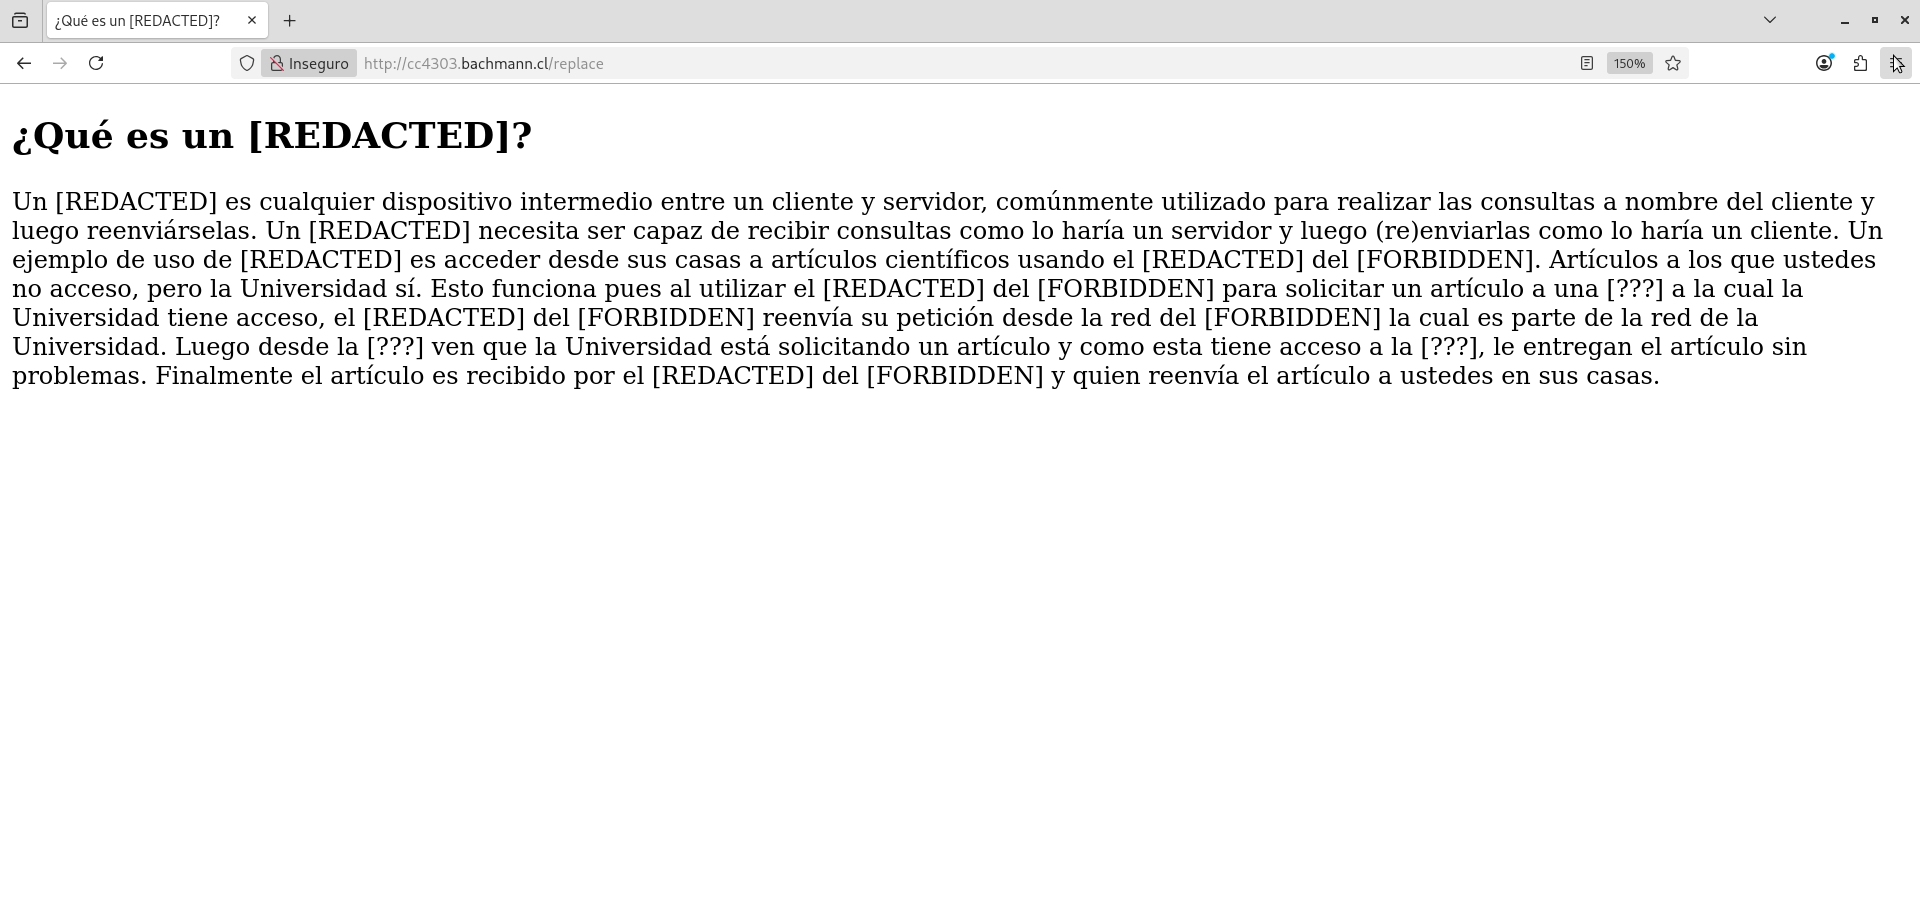
\includegraphics[width=0.8\textwidth]{img/replace.png}
		      \caption{Palabras prohibidas reemplazadas en el BODY de la respuesta.}
		      \label{fig:replace}
	      \end{figure}

\end{enumerate}

\subsection{Pruebas con buffer de recepción pequeño}
Para estas pruebas se redujo el parámetro \code{buff\_size} de \code{HttpMessage.\_read\_raw} y \code{HttpMessage.receive} (4096 por defecto) y se repitió la petición a \code{/replace}, cuya respuesta mide 1351 bytes: 17 bytes de start line, 196 bytes de área de headers y 1155 bytes de BODY.

\begin{enumerate}
	\item \textbf{Buffer de recepción menor que el mensaje pero mayor que el área de headers}
	      (\code{buff\_size = 512}): los headers se completan en una sola llamada a \code{recv()},
	      que además arrastra parte del BODY, y el BODY se completa con 2 lecturas adicionales
	      hasta alcanzar los 1155 bytes indicados por \hdr{Content-Length}
	      (Figura~\ref{fig:buffer512}).

	      \begin{figure}[H]
		      \centering
		      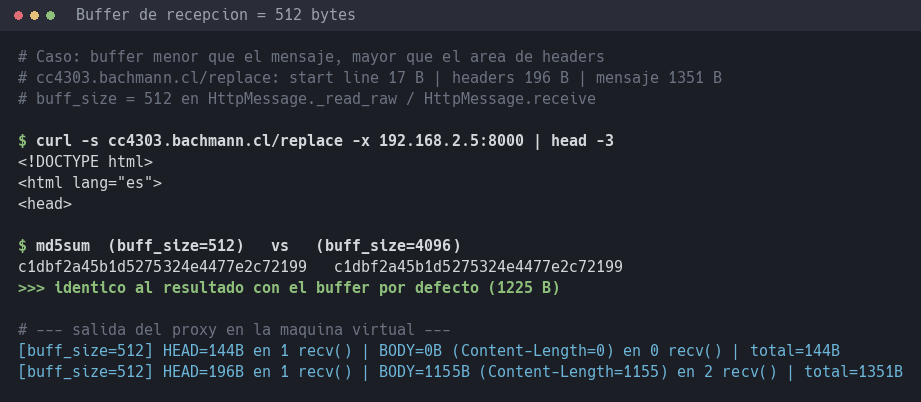
\includegraphics[width=0.8\textwidth]{img/buffer-512.png}
		      \caption{Recepción con \code{buff\_size = 512}: los headers caben en una lectura.}
		      \label{fig:buffer512}
	      \end{figure}

	\item \textbf{Buffer de recepción menor que el área de headers pero mayor que la start line}
	      (\code{buff\_size = 50}): el área de headers ya no cabe en una lectura y se arma
	      acumulando 4 llamadas a \code{recv()} hasta encontrar \verb|\r\n\r\n|; el BODY requiere
	      otras 24. La request del cliente, de 144 bytes, se arma a su vez con 3 lecturas
	      (Figura~\ref{fig:buffer50}).

	      \begin{figure}[H]
		      \centering
		      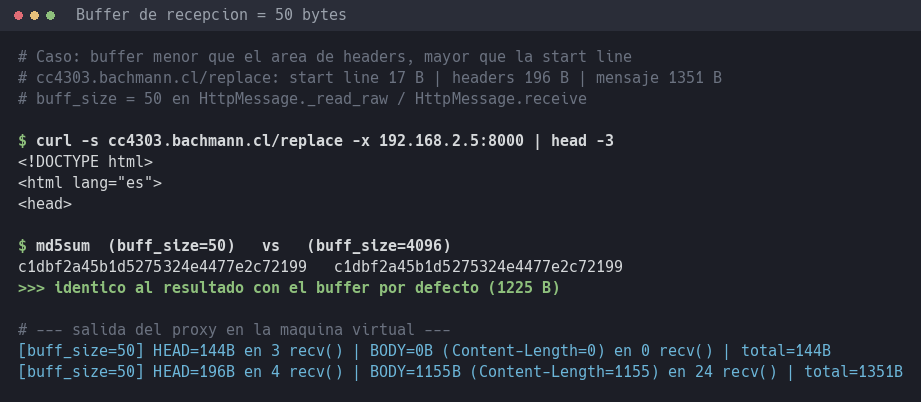
\includegraphics[width=0.8\textwidth]{img/buffer-50.png}
		      \caption{Recepción con \code{buff\_size = 50}: el área de headers requiere varias lecturas.}
		      \label{fig:buffer50}
	      \end{figure}
\end{enumerate}

En los tres tamaños probados (4096, 512 y 50) el contenido entregado al cliente fue idéntico byte a byte ---1225 bytes tras el reemplazo, mismo \code{md5sum}---, de modo que el tamaño del buffer no cambia el resultado sino solamente la cantidad de llamadas a \code{recv()}. Esto vale para respuestas delimitadas por \hdr{Content-Length}, que es el caso de \url{http://cc4303.bachmann.cl}: una respuesta \hdr{Transfer-Encoding: chunked} como la de \url{http://example.com} solo se reenvía completa mientras alcance a caber en una lectura, según la limitación ya señalada.

\section{Ejecución y repositorio}
El código se ejecuta pasando el archivo de configuración como argumento, desde el directorio del repositorio, ya que el proxy abre \code{gato.jpg} con una ruta relativa:

\begin{verbatim}
python3 server.py config.json
\end{verbatim}

El socket de escucha se enlaza a \code{(0.0.0.0, 8000)}, de modo que el proxy queda accesible en \code{IP\_VM:8000}; en las pruebas reportadas \code{IP\_VM} fue \code{192.168.2.5}. Si no se dispone de la máquina virtual, el mismo código funciona en \code{127.0.0.1:8000}.

Desde la máquina cliente, el proxy se prueba con \code{curl}:

\begin{verbatim}
curl example.com                 -x IP_VM:8000
curl cc4303.bachmann.cl          -x IP_VM:8000
curl cc4303.bachmann.cl/replace  -x IP_VM:8000
curl cc4303.bachmann.cl/secret   -x IP_VM:8000
\end{verbatim}

Para usarlo desde el navegador (Firefox) se entra a \textit{Ajustes}, sección \textit{Red}, botón \textit{Configuración}, y se elige \textit{Configuración manual del proxy}, indicando \code{IP\_VM} como \textit{Proxy HTTP} y \code{8000} como puerto. No debe marcarse la opción de usar el mismo proxy para HTTPS, ya que el proxy solo maneja HTTP.

Repositorio: \url{https://github.com/MFSaavedra/C1_Redes}

\section{Declaración de uso de IA}
En la elaboración de este informe se utilizaron modelos de inteligencia artificial para editar el template de latex, organizar secciones y traspasar a un grafo de \textit{graphviz} la figura \ref{img:proxy}. Se utilizaron \textbf{Gemini} y \textbf{Claude} (Opus 5).
El uso se limitó a:
\begin{itemize}
	\item Aclarar conceptos relacionados con el formato de HTTP y HTML.
	\item Explicar el funcionamiento de máquinas virtuales, incluyendo la configuración de puertos, modos de red (NAT, adaptador de red) y asignación de direcciones IP.
	\item Corregir/debuggear y complementar código.
\end{itemize}

Los modelos se emplearon como herramientas de consulta y explicación para comprender mejor los temas técnicos.

% FIN DEL DOCUMENTO
\end{document}
